\documentclass[11pt,a4paper]{report}
\usepackage[textwidth=37em,vmargin=30mm]{geometry}
\usepackage{calc,xunicode,amsmath,amssymb,paralist,enumitem,tabu,booktabs,datetime2,xeCJK,xeCJKfntef,listings}
\usepackage{tocloft,fancyhdr,tcolorbox,xcolor,graphicx,eso-pic,xltxtra,xelatexemoji}

\newcommand{\envyear}[0]{2025}
\newcommand{\envdatestr}[0]{2025-07-24}
\newcommand{\envfinaldir}[0]{webdb/2025/20250724/final}

\usepackage[hidelinks]{hyperref}
\hypersetup{
    colorlinks=false,
    pdfpagemode=FullScreen,
    pdftitle={Web Digest - \envdatestr}
}

\setlength{\cftbeforechapskip}{10pt}
\renewcommand{\cftchapfont}{\rmfamily\bfseries\large\raggedright}
\setlength{\cftbeforesecskip}{2pt}
\renewcommand{\cftsecfont}{\sffamily\small\raggedright}

\setdefaultleftmargin{2em}{2em}{1em}{1em}{1em}{1em}

\usepackage{xeCJK,xeCJKfntef}
\xeCJKsetup{PunctStyle=plain,RubberPunctSkip=false,CJKglue=\strut\hskip 0pt plus 0.1em minus 0.05em,CJKecglue=\strut\hskip 0.22em plus 0.2em}
\XeTeXlinebreaklocale "zh"
\XeTeXlinebreakskip = 0pt


\setmainfont{Brygada 1918}
\setromanfont{Brygada 1918}
\setsansfont{IBM Plex Sans}
\setmonofont{JetBrains Mono NL}
\setCJKmainfont{Noto Serif CJK SC}
\setCJKromanfont{Noto Serif CJK SC}
\setCJKsansfont{Noto Sans CJK SC}
\setCJKmonofont{Noto Sans CJK SC}

\setlength{\parindent}{0pt}
\setlength{\parskip}{8pt}
\linespread{1.15}

\lstset{
	basicstyle=\ttfamily\footnotesize,
	numbersep=5pt,
	backgroundcolor=\color{black!5},
	showspaces=false,
	showstringspaces=false,
	showtabs=false,
	tabsize=2,
	captionpos=b,
	breaklines=true,
	breakatwhitespace=true,
	breakautoindent=true,
	linewidth=\textwidth
}






\newcommand{\coverpic}[2]{
    % argv: itemurl, authorname
    Cover photo by #2~~(\href{#1}{#1})
}
\newcommand{\makeheader}[0]{
    \begin{titlepage}
        % \newgeometry{hmargin=15mm,tmargin=21mm,bmargin=12mm}
        \begin{center}
            
            \rmfamily\scshape
            \fontspec{BaskervilleF}
            \fontspec{Old Standard}
            \fontsize{59pt}{70pt}\selectfont
            WEB\hfill DIGEST
            
            \vfill
            % \vskip 30pt
            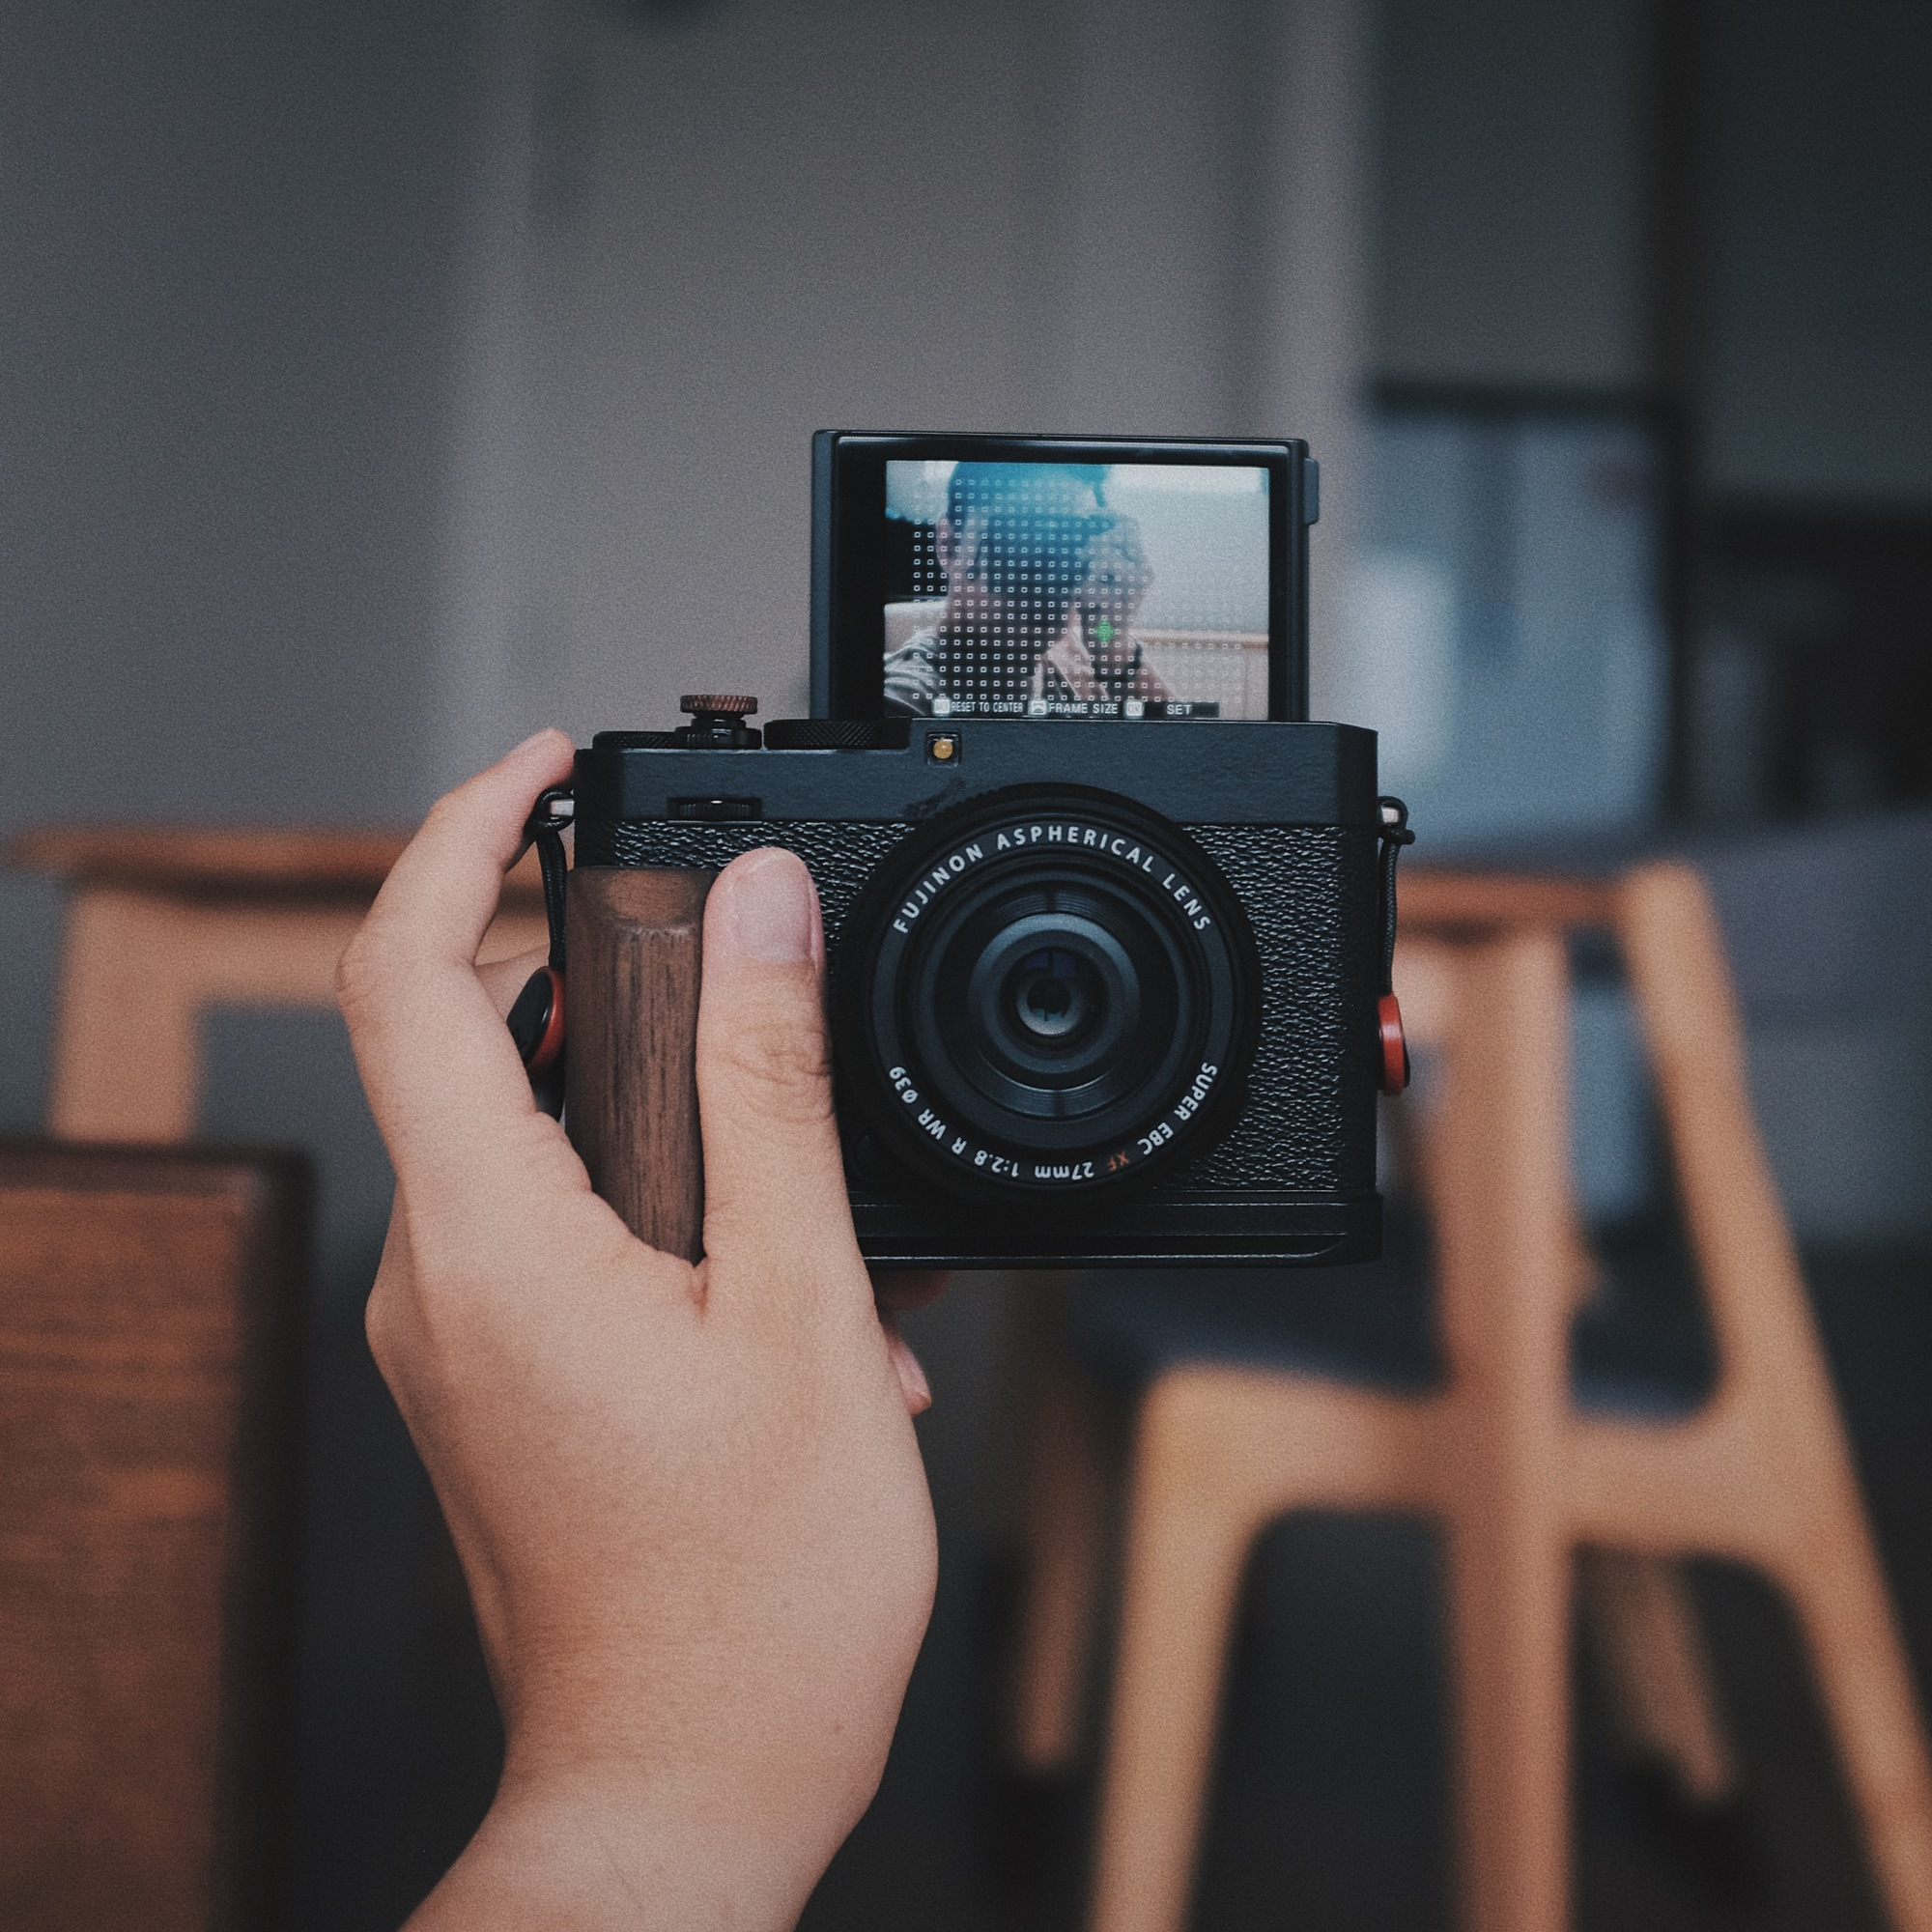
\includegraphics[width=\linewidth]{\envfinaldir/coverpic-prod.jpg}\par
            % \vskip 30pt
            \vfill

            \normalsize\rmfamily\scshape
            \copyright{} The Web Digest Project \hfill\large \envdatestr
        \end{center}
    \end{titlepage}
    % \restoregeometry
}
\newcommand{\simplehref}[1]{%
    \textcolor{blue!80!green}{\href{#1}{#1}}%
}
\renewcommand{\contentsname}{\center\Huge\sffamily\bfseries Contents\par\vskip 20pt}
\newcounter{ipartcounter}
\setcounter{ipartcounter}{0}
\newcommand{\ipart}[1]{
    % \vskip 20pt
    \clearpage
    \stepcounter{ipartcounter}
    \phantomsection
    \addcontentsline{toc}{chapter}{#1}
    % \begin{center}
    %     \Huge
    %     \sffamily\bfseries
    %     #1
    % \end{center}
    % \vskip 20pt plus 7pt
}
\newcounter{ichaptercounter}
\setcounter{ichaptercounter}{0}
\newcommand{\ichapter}[1]{
    % \vskip 20pt
    \clearpage
    \stepcounter{ichaptercounter}
    \phantomsection
    \addcontentsline{toc}{section}{\numberline{\arabic{ichaptercounter}}#1}
    \begin{center}
        \Huge
        \sffamily\bfseries
        #1
    \end{center}
    \vskip 20pt plus 7pt
}
\newcommand{\entrytitlefont}[1]{\subsection*{\raggedright\Large\sffamily\bfseries#1}}
\newcommand{\entryitemGeneric}[2]{
    % argv: title, url
    \parbox{\linewidth}{
        \entrytitlefont{#1}\par\vskip 5pt
        \footnotesize\ttfamily\mdseries
        \simplehref{#2}
    }\vskip 11pt plus 11pt minus 1pt
}
\newcommand{\entryitemGithub}[3]{
    % argv: title, url, desc
    \parbox{\linewidth}{
        \entrytitlefont{#1}\par\vskip 5pt
        \footnotesize\ttfamily\mdseries
        \simplehref{#2}\par\vskip 5pt
        \small\rmfamily\mdseries#3
    }\vskip 11pt plus 11pt minus 1pt
}
\newcommand{\entryitemAp}[3]{
    % argv: title, url, desc
    \parbox{\linewidth}{
        \entrytitlefont{#1}\par\vskip 5pt
        \footnotesize\ttfamily\mdseries
        \simplehref{#2}\par\vskip 5pt
        \small\rmfamily\mdseries#3
    }\vskip 11pt plus 11pt minus 1pt
}
\newcommand{\entryitemHackernews}[3]{
    % argv: title, hnurl, rawurl
    % \parbox{\linewidth}{
    %     \entrytitlefont{#1}\par\vskip 5pt
    %     \footnotesize\ttfamily\mdseries
    %     \simplehref{#3}\par
    %     \textcolor{black!50}{\href{#2}{#2}}
    % }\vskip 11pt plus 11pt minus 1pt
    \begin{minipage}{\linewidth}
            \entrytitlefont{#1}\par\vskip 5pt
            \footnotesize\ttfamily\mdseries
            \simplehref{#3}\par
            \textcolor{black!50}{\href{#2}{#2}}
    \end{minipage}\par\vskip 11pt plus 11pt minus 1pt
}







\begin{document}

\makeheader

\tableofcontents\clearpage




\ipart{Developers}
\ichapter{Hacker News}
\entryitemTwoLinks{I made Tinder but it's only pictures of my wife and I can only swipe right}{https://news.ycombinator.com/item?id=44664873}{https://trytender.app/}

\entryitemTwoLinks{Wife of ICEBlock app founder speaks out after DOJ fires her}{https://news.ycombinator.com/item?id=44663021}{https://www.newsweek.com/iceblock-app-founder-wife-fired-doj-carolyn-feinstein-2102214}

\entryitemTwoLinks{AccuWeather to discontinue free access to Core Weather API}{https://news.ycombinator.com/item?id=44663003}{https://developer.accuweather.com/new-portal}

\entryitemTwoLinks{Major rule about cooking meat turns out to be wrong}{https://news.ycombinator.com/item?id=44662757}{https://www.seriouseats.com/meat-resting-science-11776272}

\entryitemTwoLinks{How to increase your surface area for luck}{https://news.ycombinator.com/item?id=44662690}{https://usefulfictions.substack.com/p/how-to-increase-your-surface-area}

\entryitemTwoLinks{Employee – CEO pay gap historically wide}{https://news.ycombinator.com/item?id=44662542}{https://www.cnn.com/2025/07/23/business/afl-cio-executive-paywatch-report}

\entryitemTwoLinks{CARA – High precision robot dog using rope}{https://news.ycombinator.com/item?id=44661846}{https://www.aaedmusa.com/projects/cara}

\entryitemTwoLinks{The Promised LAN}{https://news.ycombinator.com/item?id=44661682}{https://tpl.house/}

\entryitemTwoLinks{You can now disable all AI features in Zed}{https://news.ycombinator.com/item?id=44660519}{https://zed.dev/blog/disable-ai-features}

\entryitemTwoLinks{Neil Armstrong's customs form for moon rocks (2016)}{https://news.ycombinator.com/item?id=44660437}{https://magazine.uc.edu/editors\_picks/recent\_features/armstrong/moonrocks.html}

\entryitemTwoLinks{US AI Action Plan}{https://news.ycombinator.com/item?id=44660323}{https://www.ai.gov/action-plan}

\entryitemTwoLinks{Building better AI tools}{https://news.ycombinator.com/item?id=44659921}{https://hazelweakly.me/blog/stop-building-ai-tools-backwards/}

\entryitemTwoLinks{Proxmox Donates €10k to the Perl and Raku Foundation}{https://news.ycombinator.com/item?id=44659822}{https://www.perl.com/article/proxmox-donates-to-tprf/}

\entryitemTwoLinks{Why Elixir? Common misconceptions}{https://news.ycombinator.com/item?id=44659251}{https://matthewsinclair.com/blog/0181-why-elixir}

\entryitemTwoLinks{What to expect from Debian/Trixie}{https://news.ycombinator.com/item?id=44659019}{https://michael-prokop.at/blog/2025/07/20/what-to-expect-from-debian-trixie-newintrixie/}

\entryitemTwoLinks{Reverse engineering GitHub Actions cache to make it fast}{https://news.ycombinator.com/item?id=44658909}{https://www.blacksmith.sh/blog/cache}

\entryitemTwoLinks{Cops say criminals use a Google Pixel with GrapheneOS – I say that's freedom}{https://news.ycombinator.com/item?id=44658908}{https://www.androidauthority.com/why-i-use-grapheneos-on-pixel-3575477/}

\entryitemTwoLinks{20 years of Linux on the Desktop (part 4)}{https://news.ycombinator.com/item?id=44658770}{https://ploum.net/2025-07-23-linux\_desktop4.html}

\entryitemTwoLinks{Apple's Liquid Glass: When Aesthetics Beat Function}{https://news.ycombinator.com/item?id=44658103}{https://www.maxvanijsselmuiden.nl/liquid-glass}

\entryitemTwoLinks{Cerebras launches Qwen3-235B, achieving 1.5k tokens per second}{https://news.ycombinator.com/item?id=44657727}{https://www.cerebras.ai/press-release/cerebras-launches-qwen3-235b-world-s-fastest-frontier-ai-model-with-full-131k-context-support}


\ipart{Developers~~~~(zh-Hans)}
\ichapter{Solidot}
\entryitemGeneric{\hskip 0pt{}Brave 浏览器默认屏蔽 Microsoft Recall}{https://www.solidot.org/story?sid=81869}

\entryitemGeneric{\hskip 0pt{}10\%-25\% 的肺癌患者从未吸烟}{https://www.solidot.org/story?sid=81868}

\entryitemGeneric{\hskip 0pt{}研究发现 AI 摘要会显著降低搜索结果页的点击率}{https://www.solidot.org/story?sid=81867}

\entryitemGeneric{\hskip 0pt{}微软从 Google DeepMind 挖走了至少 24 名 AI 工程师}{https://www.solidot.org/story?sid=81866}

\entryitemGeneric{\hskip 0pt{}NASA 如何从 8 亿公里外拯救朱诺号的相机}{https://www.solidot.org/story?sid=81865}

\entryitemGeneric{\hskip 0pt{}法庭裁决 Mike Lynch 的遗产以及商业伙伴欠惠普 9.44 亿美元 }{https://www.solidot.org/story?sid=81864}

\entryitemGeneric{\hskip 0pt{}阿里巴巴发布 Qwen3-Coder}{https://www.solidot.org/story?sid=81863}

\entryitemGeneric{\hskip 0pt{}乐观主义者是相似的但悲观主义者是不同的}{https://www.solidot.org/story?sid=81862}

\entryitemGeneric{\hskip 0pt{}Firefox 141 释出}{https://www.solidot.org/story?sid=81861}

\entryitemGeneric{\hskip 0pt{}科学家利用月球土壤取水}{https://www.solidot.org/story?sid=81860}

\entryitemGeneric{\hskip 0pt{}參宿四发现有一颗小伴星}{https://www.solidot.org/story?sid=81859}

\entryitemGeneric{\hskip 0pt{}Replit 删除生产数据库,伪造数据以隐藏 bug}{https://www.solidot.org/story?sid=81858}

\entryitemGeneric{\hskip 0pt{}OpenAI 和 Google DeepMind 先后宣称他们的 AI 模型在国际数学奥林匹克竞赛中取得金牌成绩}{https://www.solidot.org/story?sid=81857}

\entryitemGeneric{\hskip 0pt{}NASA X-59 Quess 低音爆超音速飞机开始滑行测试}{https://www.solidot.org/story?sid=81856}

\entryitemGeneric{\hskip 0pt{}弱密码导致一家没有备份的 158 年英国公司倒闭}{https://www.solidot.org/story?sid=81855}

\entryitemGeneric{\hskip 0pt{}研究发现四天工作制显著提升幸福感}{https://www.solidot.org/story?sid=81854}

\entryitemGeneric{\hskip 0pt{}英国考虑对苹果 iCloud 加密后门的要求做出让步}{https://www.solidot.org/story?sid=81853}

\entryitemGeneric{\hskip 0pt{}微软和法国合作创造数字版巴黎圣母院}{https://www.solidot.org/story?sid=81852}

\entryitemGeneric{\hskip 0pt{}恶意软件包上传到 Arch Linux AUR}{https://www.solidot.org/story?sid=81851}

\entryitemGeneric{\hskip 0pt{}中国证明开放权重模型比 GPU 更有效}{https://www.solidot.org/story?sid=81850}\ichapter{V2EX}
\entryitemGeneric{\hskip 0pt{}[iOS] 我发现 手记 app 的面容解锁经常自己就没了}{https://www.v2ex.com/t/1147269}

\entryitemGeneric{\hskip 0pt{}[分享创造] \#1 Flux AI:革命性的 AI 图像生成与编辑平台}{https://www.v2ex.com/t/1147268}

\entryitemGeneric{\hskip 0pt{}[问与答] 多年经验的全栈工程师,在深圳要 25k,高吗?}{https://www.v2ex.com/t/1147267}

\entryitemGeneric{\hskip 0pt{}[宽带症候群] 自己做了个查询本地和国际线路 ip 的网站}{https://www.v2ex.com/t/1147266}

\entryitemGeneric{\hskip 0pt{}[美酒与美食] 被麦当劳的 '单点不送' 谢绝订餐 感叹再也回不去了}{https://www.v2ex.com/t/1147265}

\entryitemGeneric{\hskip 0pt{}[酷工作] [远程居家办公] 招聘 Unity 开发 / 后端开发 / 测试工程师(偏后端测试)}{https://www.v2ex.com/t/1147264}

\entryitemGeneric{\hskip 0pt{}[分享创造] ImgMCP 更新:新增创作画布,支持新模型(Midjourney V1 / Seedream 3.0 等)}{https://www.v2ex.com/t/1147262}

\entryitemGeneric{\hskip 0pt{}[宽带症候群] 电信说要停我宽带了。}{https://www.v2ex.com/t/1147261}

\entryitemGeneric{\hskip 0pt{}[微信] 突然发现微信输入法全键盘双拼有一定的智能纠错能力了,当然跟 gboard 还是有一定的差距}{https://www.v2ex.com/t/1147260}

\entryitemGeneric{\hskip 0pt{}[问与答] (右甲状腺穿刺细胞液基细胞学)片内见甲状腺滤泡上皮,考虑 VI 类(甲状腺乳头状癌)—严重吗?这是松山湖中学医院出的活检结果,深圳东莞地区哪家医院对甲状腺疾病诊疗相对专业?求业内朋友告知🙏谢谢!}{https://www.v2ex.com/t/1147259}

\entryitemGeneric{\hskip 0pt{}[宽带症候群] 江苏电信似乎对美西限速了}{https://www.v2ex.com/t/1147258}

\entryitemGeneric{\hskip 0pt{}[分享发现] 用 AI 帮助别人做网站的网站 Lovable 8 个月时间 ARR 突破 1 亿美元,而国内大家只会问,这年头还有人用网站吗?}{https://www.v2ex.com/t/1147255}

\entryitemGeneric{\hskip 0pt{}[宽带症候群] 厦门移动使用第三方路由器均无法获取 IPv6, 光猫拨号正常}{https://www.v2ex.com/t/1147254}

\entryitemGeneric{\hskip 0pt{}[生活] 大半夜有人拿钥匙开我家门}{https://www.v2ex.com/t/1147253}

\entryitemGeneric{\hskip 0pt{}[创业组队] AI+康复项目出海加拿大,寻找合伙人}{https://www.v2ex.com/t/1147251}

\entryitemGeneric{\hskip 0pt{}[问与答] 大 A 和港股进入政策牛市了嘛?这次会持久多久呢?}{https://www.v2ex.com/t/1147250}

\entryitemGeneric{\hskip 0pt{}[Claude] visa 卡支付问题}{https://www.v2ex.com/t/1147249}

\entryitemGeneric{\hskip 0pt{}[V2EX] 我发现一个 BUG,我之前绑定 V2EX 用的 OKX,但是今天我打赏的时候自动使用了 phantom,没有显示我可以切换钱包插件。导致我的打赏记录不能记录到账号。}{https://www.v2ex.com/t/1147248}

\entryitemGeneric{\hskip 0pt{}[分享创造] SolVanityCL:快速生成你想要的 Sol 地址(靓号)}{https://www.v2ex.com/t/1147247}

\entryitemGeneric{\hskip 0pt{}[杭州] 关于杭州臭水官方定论 还是有点没搞懂}{https://www.v2ex.com/t/1147246}

\entryitemGeneric{\hskip 0pt{}[创业组队] [广州] 招技术(合伙人)| 有工资 | 中台平台项目已起步,缺主力开发}{https://www.v2ex.com/t/1147245}

\entryitemGeneric{\hskip 0pt{}[分享创造] 我给 Poixe 社区搭建的 Discourse 论坛,加入了 AI 机器人 [图图]}{https://www.v2ex.com/t/1147244}

\entryitemGeneric{\hskip 0pt{}[分享创造] 阿里云 ESA 边缘函数转发代理 docker registry}{https://www.v2ex.com/t/1147243}

\entryitemGeneric{\hskip 0pt{}[程序员] 面个小小厂,问一堆性能优化问题,你们厂天天搞性能优化吗?}{https://www.v2ex.com/t/1147242}

\entryitemGeneric{\hskip 0pt{}[加密货币] 有推荐的硬件钱包吗?}{https://www.v2ex.com/t/1147241}

\entryitemGeneric{\hskip 0pt{}[Apple] 苹果推出 Apple Care One}{https://www.v2ex.com/t/1147240}

\entryitemGeneric{\hskip 0pt{}[优惠信息] 免费兑换的 Train Pro}{https://www.v2ex.com/t/1147239}

\entryitemGeneric{\hskip 0pt{}[问与答] 在 openlist/alist 里添加迅雷云盘存储 貌似异地不行?}{https://www.v2ex.com/t/1147238}

\entryitemGeneric{\hskip 0pt{}[程序员] 给日本同事送了一把国产键盘,他被香哭了}{https://www.v2ex.com/t/1147237}

\entryitemGeneric{\hskip 0pt{}[Linux] Linux 上使用 iscsi-initiator-utils 作为 initiator 如何设置更大的超时时间?}{https://www.v2ex.com/t/1147236}

\entryitemGeneric{\hskip 0pt{}[游戏] 战至巅峰第四季选手用的什么手机}{https://www.v2ex.com/t/1147235}

\entryitemGeneric{\hskip 0pt{}[问与答] 特来取经 今天面试被问及 你是通过哪些渠道去获取 AI 相关最新技术和理念的,大佬们畅所欲言}{https://www.v2ex.com/t/1147234}

\entryitemGeneric{\hskip 0pt{}[问与答] Trae 2.0 SOLO 模式有人用过吗?看 b 站视频感觉很牛}{https://www.v2ex.com/t/1147232}

\entryitemGeneric{\hskip 0pt{}[分享创造] 可能是最优雅的免费无广的在线设备检测工具网站了}{https://www.v2ex.com/t/1147231}

\entryitemGeneric{\hskip 0pt{}[全球工单系统] CS2 官匹服务器挂了?提示"正在连接到 反恐精英 网络"。}{https://www.v2ex.com/t/1147230}

\entryitemGeneric{\hskip 0pt{}[NAS] 求 nas 镜像下载。点所有套件,就显示 连接失败。请检查您的网络和时间设置。}{https://www.v2ex.com/t/1147229}

\entryitemGeneric{\hskip 0pt{}[分享创造] 朋友们,新产品上线,求帮忙投一票,谢谢啦~🙏}{https://www.v2ex.com/t/1147228}

\entryitemGeneric{\hskip 0pt{}[全球工单系统] B 站直播业务挂了}{https://www.v2ex.com/t/1147227}

\entryitemGeneric{\hskip 0pt{}[微信] 腾讯 OA 宕机了?}{https://www.v2ex.com/t/1147226}

\entryitemGeneric{\hskip 0pt{}[程序员] Win11 系统下, mihomo(Clash), tun 模式生成的 Meta 接口,在 VmwareWorkstation 中的网络配置,桥接是看不到这个接口的,那么是否有变通的方式让其下虚拟机,用上这个 tun 接口?}{https://www.v2ex.com/t/1147225}

\entryitemGeneric{\hskip 0pt{}[问与答] 想 diy 台式机 有没有大佬看下应该怎么选配置}{https://www.v2ex.com/t/1147224}

\entryitemGeneric{\hskip 0pt{}[Apple] 免费领取 6 个月 50G iCloud}{https://www.v2ex.com/t/1147223}

\entryitemGeneric{\hskip 0pt{}[Android] Vivo 手机的自动调节亮度是不是很傻?}{https://www.v2ex.com/t/1147222}

\entryitemGeneric{\hskip 0pt{}[.NET] csharp 这回真成了脚本语言: dotnet run app.cs}{https://www.v2ex.com/t/1147221}

\entryitemGeneric{\hskip 0pt{}[问与答] [经验求助] 笔记本电脑连不上网如何解决?网络适配器 9560 显示叹号}{https://www.v2ex.com/t/1147220}

\entryitemGeneric{\hskip 0pt{}[程序员] odoo 这个开源程序如何啊? 是否推荐入坑, Python 理论上来说 语法和英文最接近了?}{https://www.v2ex.com/t/1147219}

\entryitemGeneric{\hskip 0pt{}[游戏] 评价下 明末:渊虚之羽}{https://www.v2ex.com/t/1147218}

\entryitemGeneric{\hskip 0pt{}[问与答] 下载 Google play 免费应用的 apk 安装包,有哪些方便的渠道?}{https://www.v2ex.com/t/1147217}

\entryitemGeneric{\hskip 0pt{}[囧] 有人快递写错手机号,如何联系上他?}{https://www.v2ex.com/t/1147216}

\entryitemGeneric{\hskip 0pt{}[酷工作] [北京] 字节番茄小说招聘后端研发工程师}{https://www.v2ex.com/t/1147215}


\ipart{Generic News}







\clearpage
\leavevmode\vfill
\footnotesize

Copyright \copyright{} 2023-2025 Neruthes and other contributors.

This document is published with CC BY-NC-ND 4.0 license.

The entries listed in this newsletter may be copyrighted by their respective creators.

This newsletter is generated by the Web Digest project.

The newsletters are also delivered via Telegram channel \CJKunderline{\href{https://t.me/webdigestchannel}{https://t.me/webdigestchannel}}.\\
RSS feed is available at \CJKunderline{\href{https://webdigest.pages.dev/rss.xml}{https://webdigest.pages.dev/rss.xml}}.

This newsletter is available in PDF at
\CJKunderline{\href{https://webdigest.pages.dev/}{https://webdigest.pages.dev/}}.

The source code being used to generate this newsletter is available at\\
\CJKunderline{\href{https://github.com/neruthes/webdigest}{https://github.com/neruthes/webdigest}}.

This newsletter is also available in
\CJKunderline{\href{http://webdigest.pages.dev/readhtml/\envyear/WebDigest-20250724.html}{HTML}} and
\CJKunderline{\href{https://github.com/neruthes/webdigest/blob/master/markdown/\envyear/WebDigest-20250724.md}{Markdown}}.


\coverpic{https://unsplash.com/photos/abstract-curves-and-light-create-a-captivating-composition-fBHi6X6B4tA}{Pawel Czerwinski}


\end{document}
